\section{MATERIAIS E MÉTODOS}

\subsection{Materiais Utilizados}

Para o experimento foram utilizados os seguintes materiais e equipamentos:
\begin{itemize}
    \item Gerador de ondas/sinais;
    \item Mola helicoidal (longitudinal);
    \item Suporte de ferro;
    \item Mufas embutidas;
    \item Pinça com mufa;
    \item Dinamômetro;
    \item Estroboscópio;
    \item Haste para suporte;
    \item Suporte para mola (acoplado à haste);
    \item Trena.
\end{itemize}

\subsection{Procedimentos Experimentais}

A montagem experimental foi configurada para a geração e observação de ondas longitudinais estacionárias em uma mola. Um suporte de ferro foi conectado ao gerador de ondas utilizando mufas. Na parte superior do suporte, uma pinça com mufa foi acoplada, à qual um dinamômetro de 2N foi preso. Uma extremidade da mola foi fixada ao pino do gerador de ondas, enquanto a outra extremidade foi conectada ao dinamômetro. A figura \ref{fig:esquema} ilustra o esquema.

\begin{figure}[H]
    \centering
    \caption{Esquema do sistema de ondas longitudinais}
    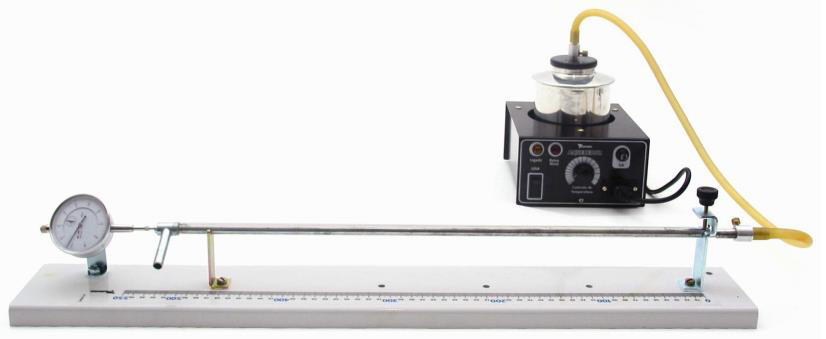
\includegraphics[width=0.15\linewidth]{figuras/esquema.png}
    \label{fig:esquema}
    \fonte{\citeonline{roteiro}}
\end{figure}

O gerador foi configurado para operar como gerador de sinais, com a chave seletora ajustada para a tensão local. Um estroboscópio foi conectado ao gerador de sinais e fixado em uma haste para auxiliar na visualização do fenômeno.



\subsubsection*{Parte I: Definição da Tensão e Observação dos Modos de Vibração}

O procedimento iniciou com a definição de uma tensão inicial na mola por meio do dinamômetro, o que estabeleceu uma altura específica para a mola. Após esta definição, uma mufa com suporte para mola foi acoplada à haste, e a mola foi presa nesse suporte no ponto correspondente à altura desejada, fixando o comprimento efetivo da mola para as medições.

Com o sistema ligado e funcionando, o volume foi ajustado enquanto a frequência do gerador de sinais era variada. Este ajuste permitiu a observação da formação de ondas estacionárias e a identificação dos nós e ventres. 

\subsubsection*{Parte II: Coleta de Dados para Diferentes Tensões}

O experimento foi conduzido para, no mínimo, duas tensões distintas na mola ($T_1$ e $T_2$). Para cada tensão definida, a mola foi fixada através do suporte. Em cada uma dessas condições de tensão, a frequência de ressonância ($F_n$) foi determinada para os diferentes modos de vibração observados. Durante o processo, foi observada a relação entre a variação da tensão e o número de nós formados.

Os dados de frequência de ressonância ($F_n$) e o índice do modo de vibração ($n$) foram registrados em tabelas separadas para cada tensão. Cada entrada da tabela incluiu um esboço da forma da onda observada para o modo correspondente.

% \subsubsection*{Parte III: Análise de Dados Preliminar}

A análise dos dados envolveu a construção de gráficos de $F_n$ versus $n$ para cada uma das tensões ($T_1$ e $T_2$), sendo ambas as curvas plotadas no mesmo gráfico para comparação. A determinação da velocidade de propagação da onda ($v$) para cada tensão foi realizada a partir da análise desses gráficos, empregando a técnica de regressão linear para extrair a inclinação da reta, que está diretamente relacionada à velocidade de propagação.